\PassOptionsToPackage{unicode=true}{hyperref} % options for packages loaded elsewhere
\PassOptionsToPackage{hyphens}{url}
%
\documentclass[]{article}
\usepackage{lmodern}
\usepackage{amssymb,amsmath}
\usepackage{ifxetex,ifluatex}
\usepackage{fixltx2e} % provides \textsubscript
\ifnum 0\ifxetex 1\fi\ifluatex 1\fi=0 % if pdftex
  \usepackage[T1]{fontenc}
  \usepackage[utf8]{inputenc}
  \usepackage{textcomp} % provides euro and other symbols
\else % if luatex or xelatex
  \usepackage{unicode-math}
  \defaultfontfeatures{Ligatures=TeX,Scale=MatchLowercase}
\fi
% use upquote if available, for straight quotes in verbatim environments
\IfFileExists{upquote.sty}{\usepackage{upquote}}{}
% use microtype if available
\IfFileExists{microtype.sty}{%
\usepackage[]{microtype}
\UseMicrotypeSet[protrusion]{basicmath} % disable protrusion for tt fonts
}{}
\IfFileExists{parskip.sty}{%
\usepackage{parskip}
}{% else
\setlength{\parindent}{0pt}
\setlength{\parskip}{6pt plus 2pt minus 1pt}
}
\usepackage{hyperref}
\hypersetup{
            pdftitle={36469 Final Project},
            pdfauthor={Jerry Li (jerryl) and Raymond Li (rli3)},
            pdfborder={0 0 0},
            breaklinks=true}
\urlstyle{same}  % don't use monospace font for urls
\usepackage[margin=1in]{geometry}
\usepackage{color}
\usepackage{fancyvrb}
\newcommand{\VerbBar}{|}
\newcommand{\VERB}{\Verb[commandchars=\\\{\}]}
\DefineVerbatimEnvironment{Highlighting}{Verbatim}{commandchars=\\\{\}}
% Add ',fontsize=\small' for more characters per line
\usepackage{framed}
\definecolor{shadecolor}{RGB}{248,248,248}
\newenvironment{Shaded}{\begin{snugshade}}{\end{snugshade}}
\newcommand{\AlertTok}[1]{\textcolor[rgb]{0.94,0.16,0.16}{#1}}
\newcommand{\AnnotationTok}[1]{\textcolor[rgb]{0.56,0.35,0.01}{\textbf{\textit{#1}}}}
\newcommand{\AttributeTok}[1]{\textcolor[rgb]{0.77,0.63,0.00}{#1}}
\newcommand{\BaseNTok}[1]{\textcolor[rgb]{0.00,0.00,0.81}{#1}}
\newcommand{\BuiltInTok}[1]{#1}
\newcommand{\CharTok}[1]{\textcolor[rgb]{0.31,0.60,0.02}{#1}}
\newcommand{\CommentTok}[1]{\textcolor[rgb]{0.56,0.35,0.01}{\textit{#1}}}
\newcommand{\CommentVarTok}[1]{\textcolor[rgb]{0.56,0.35,0.01}{\textbf{\textit{#1}}}}
\newcommand{\ConstantTok}[1]{\textcolor[rgb]{0.00,0.00,0.00}{#1}}
\newcommand{\ControlFlowTok}[1]{\textcolor[rgb]{0.13,0.29,0.53}{\textbf{#1}}}
\newcommand{\DataTypeTok}[1]{\textcolor[rgb]{0.13,0.29,0.53}{#1}}
\newcommand{\DecValTok}[1]{\textcolor[rgb]{0.00,0.00,0.81}{#1}}
\newcommand{\DocumentationTok}[1]{\textcolor[rgb]{0.56,0.35,0.01}{\textbf{\textit{#1}}}}
\newcommand{\ErrorTok}[1]{\textcolor[rgb]{0.64,0.00,0.00}{\textbf{#1}}}
\newcommand{\ExtensionTok}[1]{#1}
\newcommand{\FloatTok}[1]{\textcolor[rgb]{0.00,0.00,0.81}{#1}}
\newcommand{\FunctionTok}[1]{\textcolor[rgb]{0.00,0.00,0.00}{#1}}
\newcommand{\ImportTok}[1]{#1}
\newcommand{\InformationTok}[1]{\textcolor[rgb]{0.56,0.35,0.01}{\textbf{\textit{#1}}}}
\newcommand{\KeywordTok}[1]{\textcolor[rgb]{0.13,0.29,0.53}{\textbf{#1}}}
\newcommand{\NormalTok}[1]{#1}
\newcommand{\OperatorTok}[1]{\textcolor[rgb]{0.81,0.36,0.00}{\textbf{#1}}}
\newcommand{\OtherTok}[1]{\textcolor[rgb]{0.56,0.35,0.01}{#1}}
\newcommand{\PreprocessorTok}[1]{\textcolor[rgb]{0.56,0.35,0.01}{\textit{#1}}}
\newcommand{\RegionMarkerTok}[1]{#1}
\newcommand{\SpecialCharTok}[1]{\textcolor[rgb]{0.00,0.00,0.00}{#1}}
\newcommand{\SpecialStringTok}[1]{\textcolor[rgb]{0.31,0.60,0.02}{#1}}
\newcommand{\StringTok}[1]{\textcolor[rgb]{0.31,0.60,0.02}{#1}}
\newcommand{\VariableTok}[1]{\textcolor[rgb]{0.00,0.00,0.00}{#1}}
\newcommand{\VerbatimStringTok}[1]{\textcolor[rgb]{0.31,0.60,0.02}{#1}}
\newcommand{\WarningTok}[1]{\textcolor[rgb]{0.56,0.35,0.01}{\textbf{\textit{#1}}}}
\usepackage{graphicx,grffile}
\makeatletter
\def\maxwidth{\ifdim\Gin@nat@width>\linewidth\linewidth\else\Gin@nat@width\fi}
\def\maxheight{\ifdim\Gin@nat@height>\textheight\textheight\else\Gin@nat@height\fi}
\makeatother
% Scale images if necessary, so that they will not overflow the page
% margins by default, and it is still possible to overwrite the defaults
% using explicit options in \includegraphics[width, height, ...]{}
\setkeys{Gin}{width=\maxwidth,height=\maxheight,keepaspectratio}
\setlength{\emergencystretch}{3em}  % prevent overfull lines
\providecommand{\tightlist}{%
  \setlength{\itemsep}{0pt}\setlength{\parskip}{0pt}}
\setcounter{secnumdepth}{0}
% Redefines (sub)paragraphs to behave more like sections
\ifx\paragraph\undefined\else
\let\oldparagraph\paragraph
\renewcommand{\paragraph}[1]{\oldparagraph{#1}\mbox{}}
\fi
\ifx\subparagraph\undefined\else
\let\oldsubparagraph\subparagraph
\renewcommand{\subparagraph}[1]{\oldsubparagraph{#1}\mbox{}}
\fi

% set default figure placement to htbp
\makeatletter
\def\fps@figure{htbp}
\makeatother

\usepackage{xcolor}
\usepackage{booktabs}
\usepackage{longtable}
\usepackage{array}
\usepackage{multirow}
\usepackage{wrapfig}
\usepackage{float}
\usepackage{colortbl}
\usepackage{pdflscape}
\usepackage{tabu}
\usepackage{threeparttable}
\usepackage{threeparttablex}
\usepackage[normalem]{ulem}
\usepackage{makecell}
\usepackage{xcolor}

\title{36469 Final Project}
\author{Jerry Li (jerryl) and Raymond Li (rli3)}
\date{12/6/2021}

\begin{document}
\maketitle

\hypertarget{data}{%
\section{Data}\label{data}}

The Zeisel dataset collects data on RNA sequencing for 3005 mouse cells
across 1000 genes.

\begin{verbatim}
## cell_types
## astrocytes_ependymal    endothelial-mural         interneurons 
##                  224                  235                  290 
##            microglia     oligodendrocytes        pyramidal CA1 
##                   98                  820                  939 
##         pyramidal SS 
##                  399
\end{verbatim}

We see that the dataset contains 7 types of labelled cells, with
pyramidal CA1 being the most common and microglia being the least
common.

\hypertarget{pca-clustering-analysis}{%
\section{PCA Clustering Analysis}\label{pca-clustering-analysis}}

\emph{Part B}

\includegraphics{36469-Final-Project_files/figure-latex/unnamed-chunk-5-1.pdf}

The scree plot shows four main outlier points on the upper left, where
the eiganvalues are higher than those of the rest of the data. Because
of this, it seems reasonable to only find the first four principal
component values.

The data showed by the scatterplot indicates the first two principal
components is not enough to differentiate between the cell types. It
looks like all four cell types are in the same cluster with the
exception of one data point outlier. However, four cell types should
have four distinct clusters.

\emph{Part C}

\begin{verbatim}
##    cell_types
##     astrocytes_ependymal endothelial-mural interneurons microglia
##   1                    2                 5           23         0
##   2                    0                 0            8         1
##   3                    7               223            4        90
##   4                  214                 3            4         6
##   5                    0                 0            4         0
##   6                    1                 1            0         1
##   7                    0                 3          247         0
##    cell_types
##     oligodendrocytes pyramidal CA1 pyramidal SS
##   1                0           323          279
##   2               89            43           37
##   3               17             4           10
##   4               18            18            7
##   5                0           546           64
##   6              696             0            0
##   7                0             5            2
\end{verbatim}

\begin{Shaded}
\begin{Highlighting}[]
\KeywordTok{compute_misclustering_rate}\NormalTok{(cell_types, conf_matrix}\OperatorTok{$}\NormalTok{cluster)}
\end{Highlighting}
\end{Shaded}

\begin{verbatim}
## [1] 0.2658902
\end{verbatim}

Based on the reported results, the quality of the estimated clustering
seems mediocre. While the misclustering rate is just 17 percent, cluster
2 isn't matched to a cell. On the other hand, cluster 4 is matched with
two cell types.

\emph{Part D}

\begin{verbatim}
##    cell_types
##     astrocytes_ependymal endothelial-mural interneurons microglia
##   1                    0                 2            1        93
##   2                    0                 1            4         0
##   3                    7               208            3         3
##   4                  210                 5            7         0
##   5                    1                 0           71         0
##   6                    0                 0            0         0
##   7                    6                19          204         2
##    cell_types
##     oligodendrocytes pyramidal CA1 pyramidal SS
##   1               29             2            6
##   2              151            41           33
##   3               18            15           17
##   4               27            42           13
##   5                0           557          136
##   6              593             0            0
##   7                2           282          194
\end{verbatim}

\begin{Shaded}
\begin{Highlighting}[]
\KeywordTok{length}\NormalTok{(cell_types)}
\end{Highlighting}
\end{Shaded}

\begin{verbatim}
## [1] 3005
\end{verbatim}

\begin{Shaded}
\begin{Highlighting}[]
\KeywordTok{length}\NormalTok{(conf_matrix_d}\OperatorTok{$}\NormalTok{cluster)}
\end{Highlighting}
\end{Shaded}

\begin{verbatim}
## [1] 3005
\end{verbatim}

\begin{Shaded}
\begin{Highlighting}[]
\KeywordTok{compute_misclustering_rate}\NormalTok{(cell_types, conf_matrix_d}\OperatorTok{$}\NormalTok{cluster)}
\end{Highlighting}
\end{Shaded}

\begin{verbatim}
## [1] 0.368386
\end{verbatim}

\includegraphics{36469-Final-Project_files/figure-latex/unnamed-chunk-10-1.pdf}

When comparing with Figure 2, the scatterplot gives a better result, but
barely. It seems like the red cluster (group 3) is clearly defined, but
the other three interact with eachother too much to be distinguisable.

The matrix and the misclustering rate, on the other hand, indicates a
solid clustering. The matrix shows all four clusters are paired mostly
with a unique cell type. The misclustering rate is 6.7\%, much lower
than the previous rate from part C.

\emph{Part E}

\begin{verbatim}
##  Fold  1  out of  5 
##  Fold  2  out of  5 
##  Fold  3  out of  5 
##  Fold  4  out of  5 
##  Fold  5  out of  5
\end{verbatim}

\emph{Part F}

\begin{verbatim}
##    cell_types
##     astrocytes_ependymal endothelial-mural interneurons microglia
##   1                    0                 2            1        93
##   2                    0                 0            5         0
##   3                    7               198            4         2
##   4                  206                 5            7         0
##   5                    0                 0           82         0
##   6                    0                 4            0         1
##   7                   11                26          191         2
##    cell_types
##     oligodendrocytes pyramidal CA1 pyramidal SS
##   1               34             4            6
##   2              671            16           23
##   3                4            14           14
##   4               28            45           14
##   5                0           654          160
##   6               81             0            2
##   7                2           206          180
\end{verbatim}

\begin{Shaded}
\begin{Highlighting}[]
\KeywordTok{compute_misclustering_rate}\NormalTok{(cell_types, conf_matrix_f}\OperatorTok{$}\NormalTok{cluster)}
\end{Highlighting}
\end{Shaded}

\begin{verbatim}
## [1] 0.3294509
\end{verbatim}

\includegraphics{36469-Final-Project_files/figure-latex/unnamed-chunk-15-1.pdf}

Using Sparce PCA yields better results compared to the clustering seen
in 1B and 1C. Since the features are correlated with eachother, sPCA is
beneficial by providing high factor loadings. The result is the opposite
from what we have seen, where the data points are possible too sparce
and does not cluster- rather than clustering too close and being
indistingishable from eachother.

On the other hand, the matrix and misclustering rate is still not great-
the matrix shows cluster 3 containing two cell types. The misclustering
rate is 19.4\%, higher than previously seen.

\hypertarget{xgboost-classification}{%
\section{XGBoost Classification}\label{xgboost-classification}}

XGBoost is a powerful classification model that uses gradient boosting
to outperform many other algorithms for classification.

As aforementioned, the full Zeisel dataset collects data on 3005 mouse
cells. To conduct XGBoost classification, we first randomly split the
data into training (75\%) and testing (25\%), i.e.~Leave-One-Out Cross
Validation (LOOCV), which will allow us to verify the model's findings.

\begin{verbatim}
## [17:31:43] WARNING: amalgamation/../src/learner.cc:573: 
## Parameters: { "nthreads" } might not be used.
## 
##   This may not be accurate due to some parameters are only used in language bindings but
##   passed down to XGBoost core.  Or some parameters are not used but slip through this
##   verification. Please open an issue if you find above cases.
\end{verbatim}

\begin{verbatim}
## ##### xgb.Booster
## raw: 272.9 Kb 
## call:
##   xgb.train(params = params, data = xgb.train, nrounds = 20, nthreads = 1)
## params (as set within xgb.train):
##   booster = "gbtree", eta = "0.001", max_depth = "5", gamma = "3", subsample = "0.75", colsample_bytree = "1", objective = "multi:softprob", eval_metric = "mlogloss", num_class = "7", nthreads = "1", validate_parameters = "TRUE"
## xgb.attributes:
##   niter
## callbacks:
##   cb.print.evaluation(period = print_every_n)
## # of features: 1000 
## niter: 20
## nfeatures : 1000
\end{verbatim}

We fit this XGBoost model with a learning rate of 0.001, gamma value of
3, and max depth of 5 to prevent overfitting by making the boosting
process more conservative. The booster ran for 20 rounds on the training
dataset using the \texttt{multi:softprob} model, which predicts
probabilities that an observation falls into each of the 7 cell types.
This makes use of the softmax objective function, which is described as:

\[\sigma(\overrightarrow{z})_j=\frac{e^{z_j}}{\sum_{k=1}^Ke^{z_k}}\]

The final accuracy of this model was quite high with a training error of
2.09\% and testing error of 5.98\%, which are both incredibly low. We
can further visualize the model's decisions in the figure below, which
shows the top 8 most important features in the model. The \texttt{Crym},
\texttt{Slc32a1}, \texttt{Mobp}, \texttt{Mbp}, and \texttt{Mef2c} genes
stand out as the features that produce the highest information gain,
suggesting that they are most important in determining cell type.

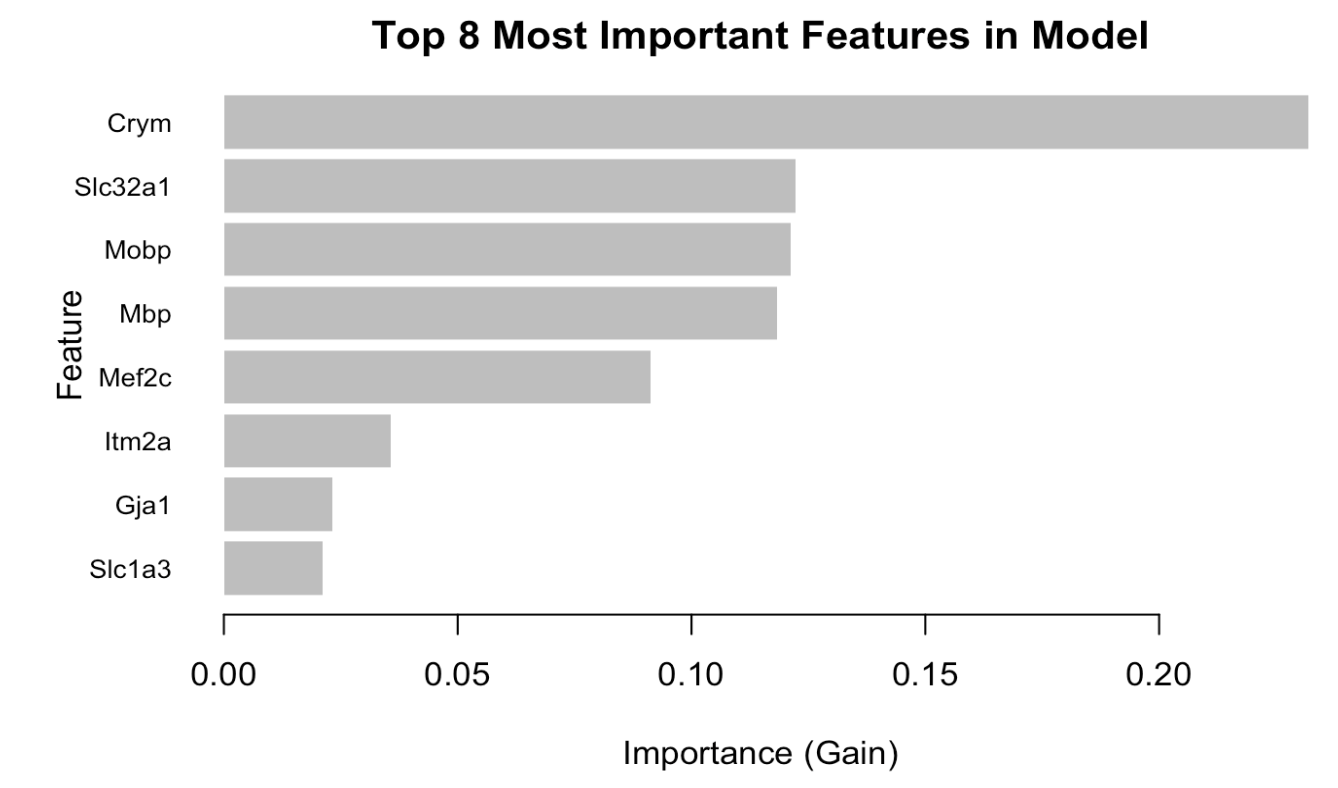
\includegraphics{Importance 1.png}

\begin{Shaded}
\begin{Highlighting}[]
\KeywordTok{xgb.plot.importance}\NormalTok{(}\DataTypeTok{importance_matrix=}\KeywordTok{xgb.importance}\NormalTok{(}\DataTypeTok{model=}\NormalTok{xgb.fit),}
                    \DataTypeTok{top_n=}\DecValTok{8}\NormalTok{,}
                    \DataTypeTok{xlab=}\StringTok{"Importance (Gain)"}\NormalTok{,}
                    \DataTypeTok{ylab=}\StringTok{"Feature"}\NormalTok{,}
                    \DataTypeTok{main=}\StringTok{"Top 8 Most Important Features in Model"}\NormalTok{)}
\end{Highlighting}
\end{Shaded}

The first XGBoost decision tree is shown below--we can see that some of
the most important features are indeed used in this tree.

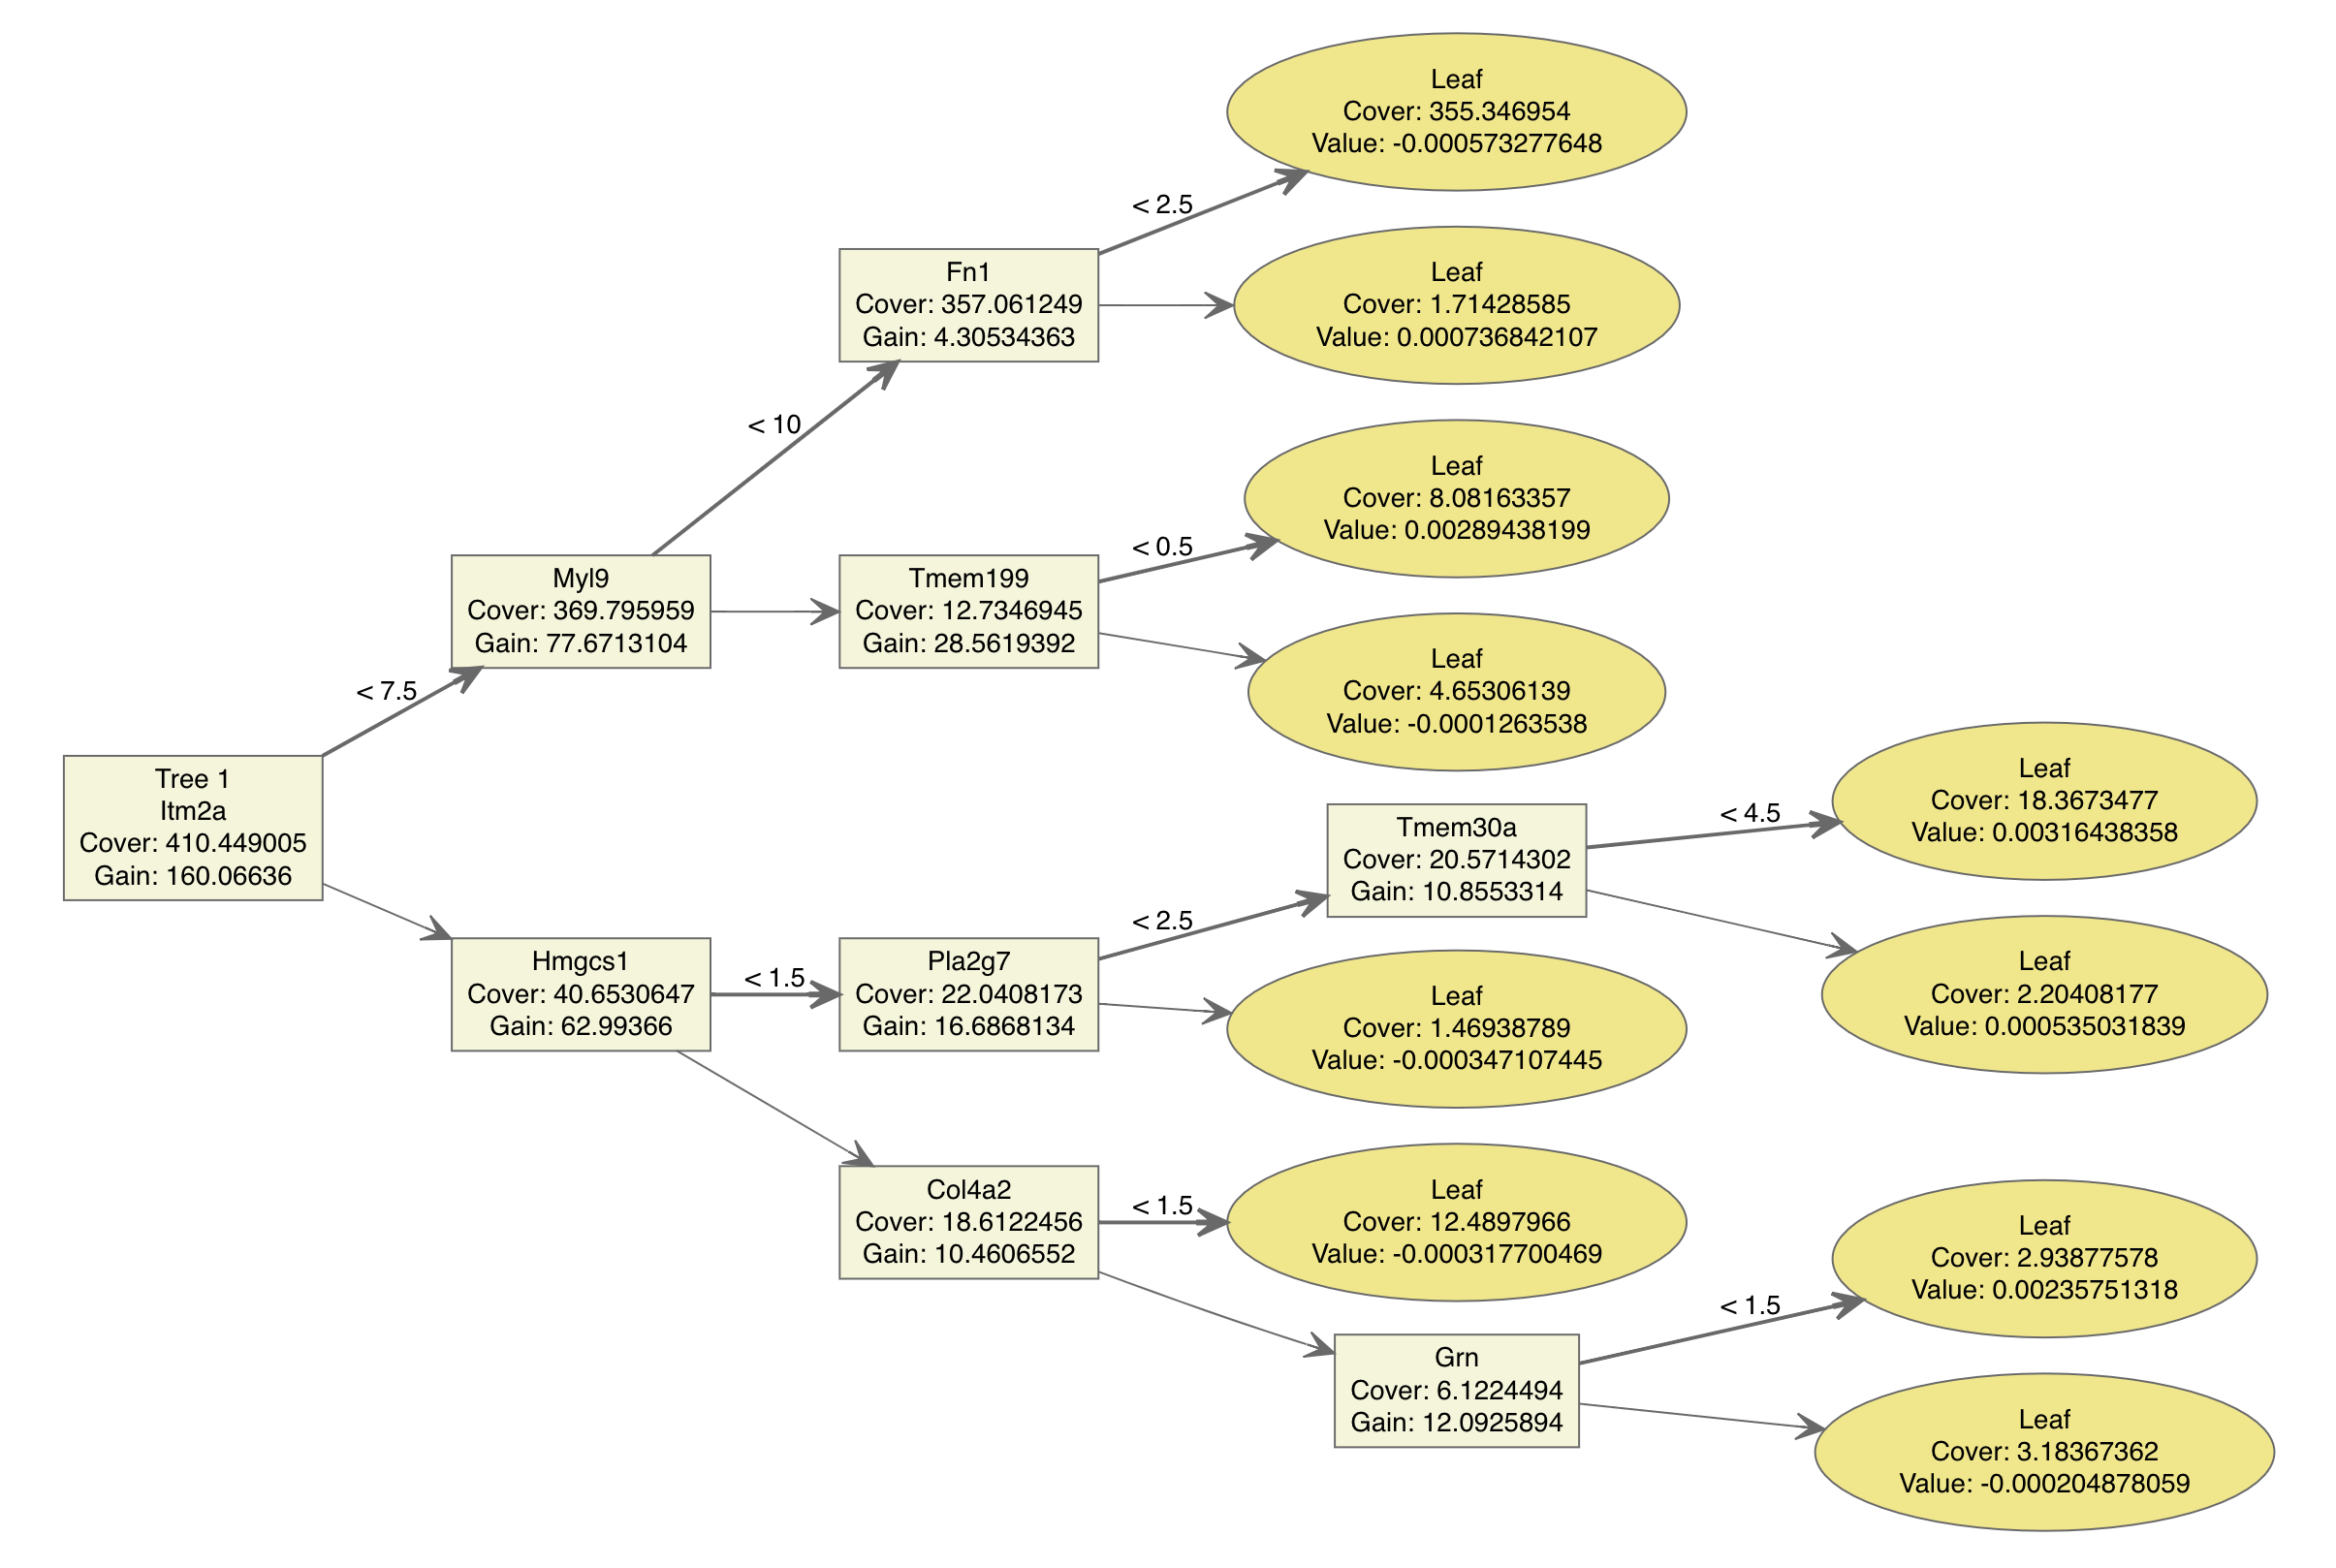
\includegraphics{Tree 1.png}

\begin{Shaded}
\begin{Highlighting}[]
\KeywordTok{library}\NormalTok{(DiagrammeR)}
\KeywordTok{xgb.plot.tree}\NormalTok{(}\DataTypeTok{model=}\NormalTok{xgb.fit,}\DataTypeTok{trees=}\DecValTok{1}\NormalTok{)}
\end{Highlighting}
\end{Shaded}

However, despite the fact that the training and testing error are both
small and have a marginal difference, the testing error is higher than
the training error. In addition, the tree supports this idea that the
model may be overfitting, as there seem to be a high number of splits
and some that seem almost arbitrary. Thus, we may choose to add an L2
regularization term of 0.1 to smooth parameters toward 0 and avoid
overfitting.

\begin{verbatim}
## [17:31:53] WARNING: amalgamation/../src/learner.cc:573: 
## Parameters: { "nthreads" } might not be used.
## 
##   This may not be accurate due to some parameters are only used in language bindings but
##   passed down to XGBoost core.  Or some parameters are not used but slip through this
##   verification. Please open an issue if you find above cases.
\end{verbatim}

\begin{verbatim}
## ##### xgb.Booster
## raw: 279.5 Kb 
## call:
##   xgb.train(params = params, data = xgb.train, nrounds = 20, nthreads = 1, 
##     lambda = 0.1)
## params (as set within xgb.train):
##   booster = "gbtree", eta = "0.001", max_depth = "5", gamma = "3", subsample = "0.75", colsample_bytree = "1", objective = "multi:softprob", eval_metric = "mlogloss", num_class = "7", nthreads = "1", lambda = "0.1", validate_parameters = "TRUE"
## xgb.attributes:
##   niter
## callbacks:
##   cb.print.evaluation(period = print_every_n)
## # of features: 1000 
## niter: 20
## nfeatures : 1000
\end{verbatim}

Interestingly, including L2 regularization produced a more significant
difference between training and testing error--we see that training
error is now 1.46\% whereas testing error is 5.98\%. While this
regularization attempt has failed, it is nonetheless interesting to
analyze the differences between the two models.

Visualizing the most important features, we observe that some of the top
8 have changed between the two models. This may be because some features
that are included at many lower splits which would provide more
information are now penalized, thereby reducing their importance in the
regularized model.

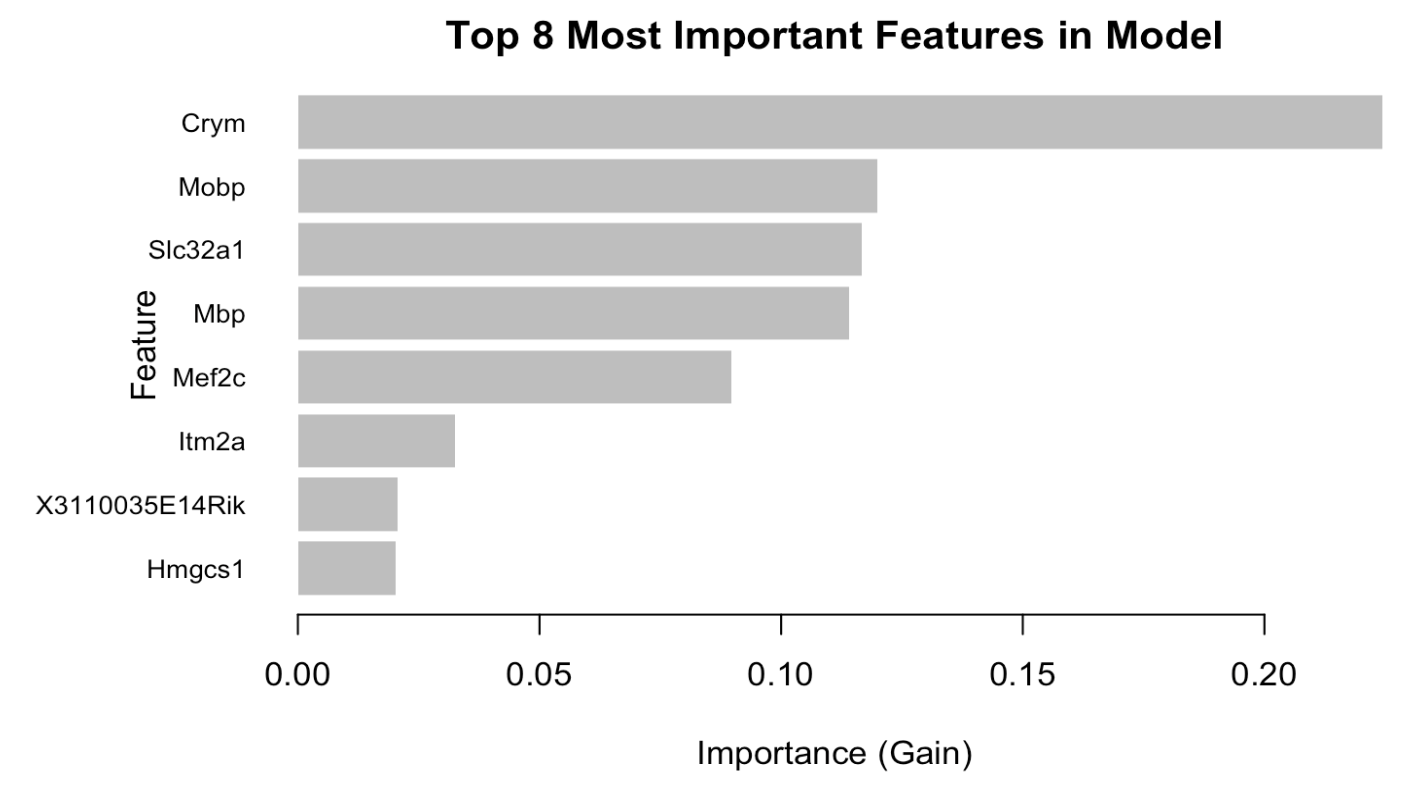
\includegraphics{Importance 2.png}

\begin{Shaded}
\begin{Highlighting}[]
\KeywordTok{xgb.plot.importance}\NormalTok{(}\DataTypeTok{importance_matrix=}\KeywordTok{xgb.importance}\NormalTok{(}\DataTypeTok{model=}\NormalTok{xgb.fit),}
                    \DataTypeTok{top_n=}\DecValTok{8}\NormalTok{,}
                    \DataTypeTok{xlab=}\StringTok{"Importance (Gain)"}\NormalTok{,}
                    \DataTypeTok{ylab=}\StringTok{"Feature"}\NormalTok{,}
                    \DataTypeTok{main=}\StringTok{"Top 8 Most Important Features in Model"}\NormalTok{)}
\end{Highlighting}
\end{Shaded}

The first decision tree, as shown below, is also interesting--the number
of splits seems to have increased, if anything, as compared to the
non-regularized model. However, this may be explained by the
coefficients on each feature shrinking toward 0 and not necessarily
being altogether eliminated from the model, which would be the case with
L1 regularization.

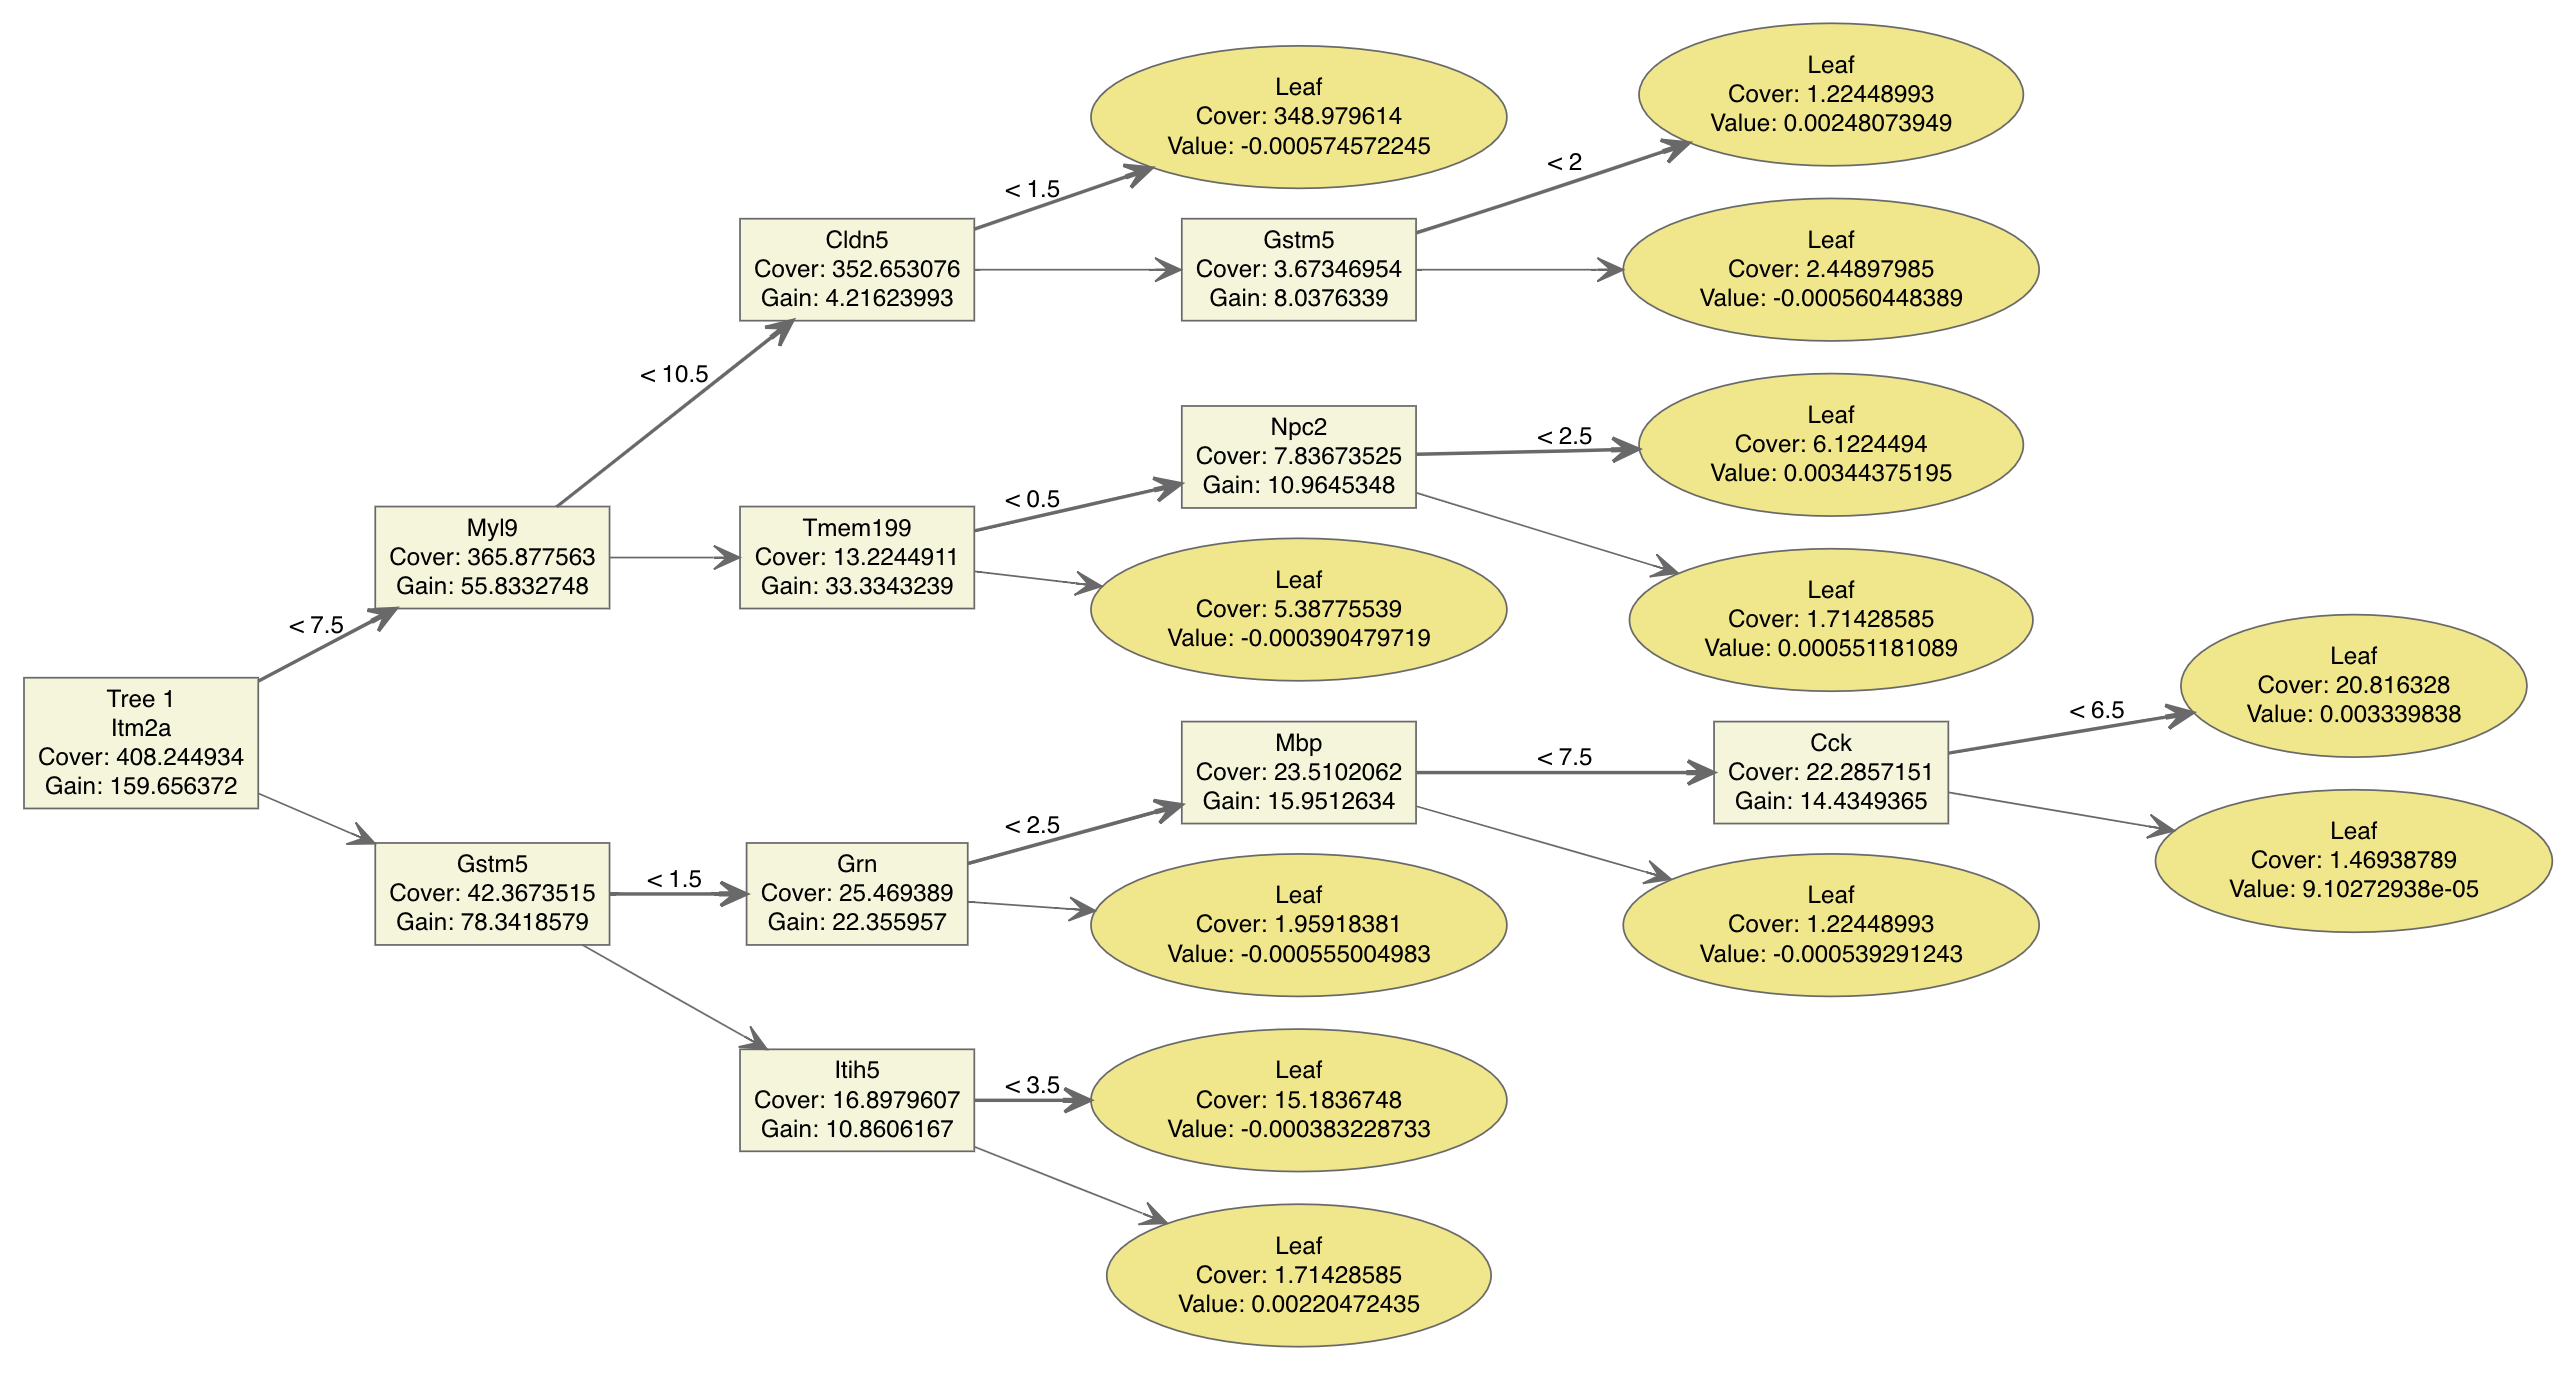
\includegraphics{Tree 2.png}

\begin{Shaded}
\begin{Highlighting}[]
\KeywordTok{library}\NormalTok{(DiagrammeR)}
\KeywordTok{xgb.plot.tree}\NormalTok{(}\DataTypeTok{model=}\NormalTok{xgb.fit,}\DataTypeTok{trees=}\DecValTok{1}\NormalTok{)}
\end{Highlighting}
\end{Shaded}

\end{document}
